\section{Periodicity}

A system is periodic if $x(t) = x(t + T)$, or 
in the case of discrete time, if $x[n] = x[n + N]$. 


% Periodic Continuous-Time Signal
\begin{figure}
    \centering
    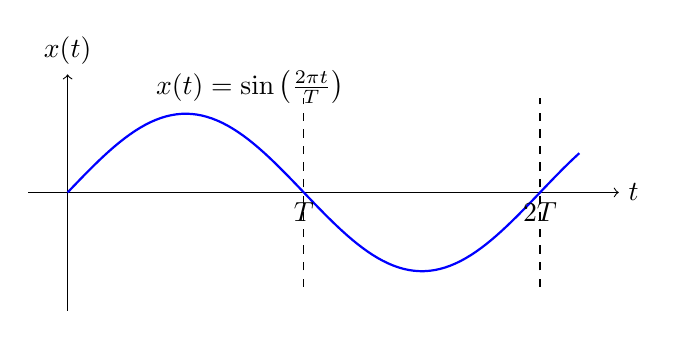
\begin{tikzpicture}[scale=1]
        % Axes
        \draw[->] (-0.5, 0) -- (7, 0) node[right] {$t$};
        \draw[->] (0, -1.5) -- (0, 1.5) node[above] {$x(t)$};
    
        \draw[thick, blue, domain=0:6.5, samples=100] plot (\x, {sin(60*\x)});
    
        % T markings
        \node[below] at (3, 0) {$T$};
        \draw[dashed] (3, -1.2) -- (3, 1.2);
        \node[below] at (6, 0) {$2T$};
        \draw[dashed] (6, -1.2) -- (6, 1.2);
    
        % Labels
        \node[above right] at (1, 1) {$x(t) = \sin\left(\frac{2\pi t}{T}\right)$};
    \end{tikzpicture}
    \caption{Periodic CT Signal}
\end{figure}
    
\begin{figure}
    \centering
    \begin{tikzpicture}[scale=1]
        % Axes
        \draw[->] (-0.5, 0) -- (7, 0) node[right] {$n$};
        \draw[->] (0, -1.5) -- (0, 1.5) node[above] {$x[n]$};
    
        % Stem plot for a cosine signal
        \foreach \n in {0, 1, ..., 7} {
            \draw[thick, blue] (\n, 0) -- (\n, {cos(60*\n)});
            \filldraw[blue] (\n, {cos(60*\n)}) circle (0.07);
        }
    
        % T markings
        \node[below] at (6, 0) {$N$};
        \draw[dashed] (6, -1.2) -- (6, 1.2);
    
        % Labels
        \node[above right] at (2, 1) {$x[n] = \cos\left(\frac{2\pi n}{N}\right)$};
    \end{tikzpicture}
    \caption{Periodic DT Signal}
\end{figure}

The fundemental period is the smallest $T_0$ (or $N_0$) such 
that $x(t) = x(t + T_0)$ (or $x[n] = x[n + N_0]$). If $x(t)$ is periodic, $x_{Re}(t) + j x_{Im}(t)$ is also 
periodic. However, if $x_1(t)$ and $x_2(t)$ are periodic then it is not 
necessarily the case that $x_1(t) + x_2(t)$ is 
periodic. Consider $x_1(t) = \sin(t)$ and 
$x_2(t) = \sin(\sqrt{2} t)$. $x_1(t) + x_2(t) = \sin(t) + \sin(\sqrt{2}t)$.
$x_1(t)$ has period $2\pi$. $x_2(t)$ has period $\frac{2\pi}{\sqrt{2}}$. 
However, their sum is not periodic and in fact the sum of 
any $x_1(t)$, $x_2(t)$ will be aperiodic when the ratio 
of their periods is irrational. 

\begin{figure}
    \centering
    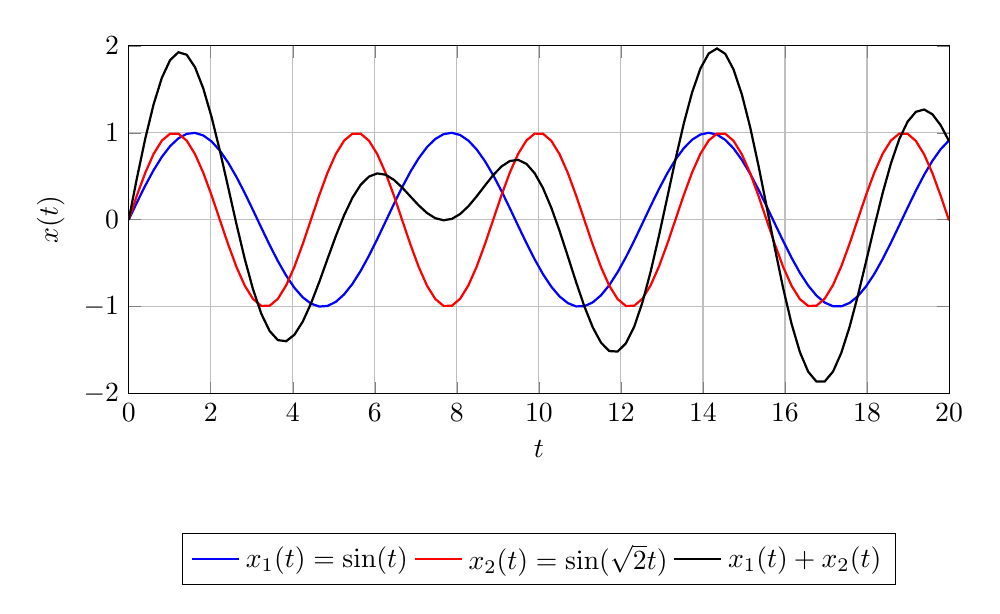
\begin{tikzpicture}
        \begin{axis}[
            width=12cm, height=6cm,
            xlabel={$t$}, ylabel={$x(t)$},
            grid=both,
            legend style={at={(0.5,-0.4)}, anchor=north, legend columns=3},
            xmin=0, xmax=20,
            ymin=-2, ymax=2,
            domain=0:20,
            samples=100
        ]
        \addplot[blue, thick] {sin(deg(x))};         
        \addlegendentry{$x_1(t) = \sin(t)$};
    
        \addplot[red, thick] {sin(sqrt(2) * deg(x))};
        \addlegendentry{$x_2(t) = \sin(\sqrt{2} t)$};
    
        \addplot[thick, black] {sin(deg(x)) + sin(deg(sqrt(2) * x))};
        \addlegendentry{$x_1(t) + x_2(t)$};
        \end{axis}
    \end{tikzpicture}
    \caption{Periodic Signals Sum}
\end{figure}
